\section{Evaluation}
\label{sec:eval}
\textbf{Methodology.} We report \emph{prototype} measurements, one cloud deployment plus a
developer workstation, as evidence of feasibility, not statistical generalization
(this is a Level-5 systems-design evaluation: an artifact exercised under controlled
conditions). Erasure and placement experiments invoke the production encoder and HRW code paths
directly rather than a re-implementation; storage figures average rendezvous placement of every
shard over $2000$ synthetic blocks per network size; throughput is the mean of $20$ encode/decode
repetitions per body size on a single core; PoW figures are medians over nine independently
generated identities to capture the geometric-distribution variance of the search. Functional and
security results come from the automated test suite and from exercising the live deployment.

\textbf{Reproducibility.} Every measurement here derives from a deterministic code path. The storage
figures are a function of $(n,K,M,r)$ and the rendezvous hash of fixed synthetic block identifiers,
so they reproduce exactly given the same parameters; the throughput numbers depend only on body size
and the single-core encoder; the PoW costs follow the geometric distribution of a fixed difficulty,
which is why we report medians over independent identities rather than a single run. The functional
and security checks are encoded as repeatable tests over the same deterministic core that runs in
production, so a reviewer with the artifact can re-derive each result without access to our specific
cloud host. We consider this the appropriate reproducibility bar for a single-team prototype, short
of the controlled multi-system benchmark we leave to future work (\S\ref{sec:disc}).

\subsection{Storage scarcity}
We instantiate the model of \S\ref{sec:storagemodel} with $1$\,MiB block bodies, the network's
adaptive $(K,M)$ and $r$, and rendezvous placement of every shard over $n$ nodes, averaged over
$2000$ blocks. Table~\ref{tab:storage} reports the bytes each node retains per block and the
reduction versus full replication. The measured reduction tracks the analytical $\rho=Kn/(Tr)$:
per-node history falls roughly as $O(1/n)$ while full replication stays at $1$\,MiB/block/node,
reaching $\approx 28\times$ at $n{=}128$ and widening thereafter. Below $n{=}4$ fragmentation is
not yet a win, as the model predicts.

\begin{table}[t]
\centering
\caption{Per-node history storage vs.\ full replication (1\,MiB blocks; rendezvous placement
averaged over 2000 blocks). ``max'' shards/node stayed within $3\%$ of the mean, confirming HRW
balance.}
\label{tab:storage}
\begin{tabular}{rlrrr}
\toprule
$n$ & spec & $r$ & store/node/blk & reduction $\rho$ \\
\midrule
4   & K3\,M1  & 2 & 683\,KiB & 1.5$\times$ \\
8   & K6\,M2  & 3 & 512\,KiB & 2.0$\times$ \\
16  & K11\,M5 & 3 & 279\,KiB & 3.7$\times$ \\
32  & K16\,M8 & 3 & 144\,KiB & 7.1$\times$ \\
64  & K16\,M8 & 3 & 72\,KiB  & 14.2$\times$ \\
128 & K16\,M8 & 3 & 36\,KiB  & 28.4$\times$ \\
256 & K16\,M8 & 3 & 18\,KiB  & 56.9$\times$ \\
\bottomrule
\end{tabular}
\end{table}

\begin{figure}[t]
\centering
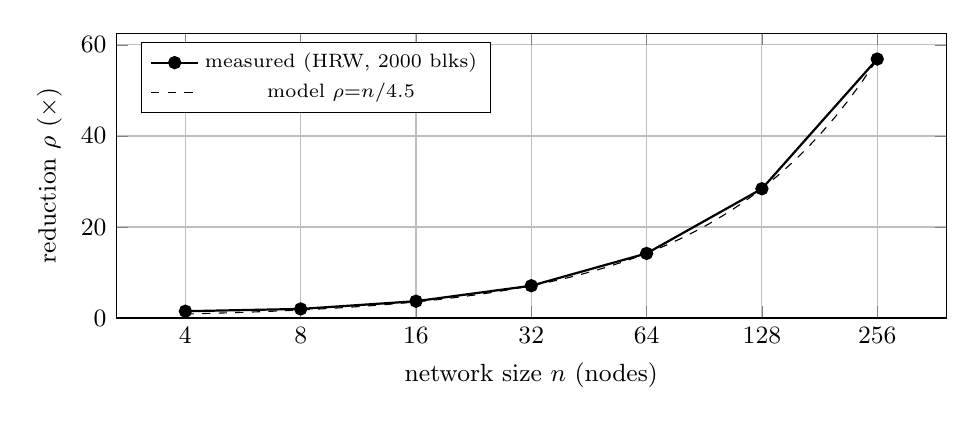
\begin{tikzpicture}
\begin{axis}[
  width=\columnwidth, height=5.2cm, font=\small,
  xlabel={network size $n$ (nodes)}, ylabel={reduction $\rho$ ($\times$)},
  xmode=log, log basis x=2, xtick={4,8,16,32,64,128,256},
  xticklabels={4,8,16,32,64,128,256},
  ymin=0, grid=both, legend pos=north west, legend style={font=\scriptsize}]
\addplot[mark=*,thick] coordinates {(4,1.5)(8,2.0)(16,3.7)(32,7.1)(64,14.2)(128,28.4)(256,56.9)};
\addlegendentry{measured (HRW, 2000 blks)}
\addplot[dashed,domain=4:256,samples=50] {x/4.5};
\addlegendentry{model $\rho{=}n/4.5$}
\end{axis}
\end{tikzpicture}
\caption{Per-node history-storage reduction vs.\ full replication. Measured rendezvous placement
tracks the analytical $\rho=Kn/(Tr)$ once the erasure shape saturates ($n\gtrsim32$).}
\label{fig:storagecurve}
\end{figure}

\subsection{Comparison with replication baselines}
Storage alone is an incomplete metric; the right comparison holds \emph{durability} fixed or
reports both. Table~\ref{tab:baseline} contrasts three schemes for a $128$-node network and
$1$\,MiB blocks: a classic full node (one whole replica per node), naive $3\times$ whole-block
replication distributed over the network, and ShadowLedger (K16\,M8, $r{=}3$). Whole-block
$3\times$ replication is actually \emph{cheaper} per node ($24$\,KiB) than ShadowLedger
($36$\,KiB), but it loses a block whenever the three holders of that block are all down
($\Pr=f^3\approx2.7\times10^{-2}$ at $f{=}0.3$), because there is no parity to recover from a
partial set. ShadowLedger spends $50\%$ more bytes to add erasure parity, buying roughly four
orders of magnitude better durability ($\Pr[\text{loss}]<10^{-6}$ at the same $f$,
\S\ref{sec:threat}) while still storing $\approx28\times$ less than a full node. The adaptive
shape also keeps the data/parity ratio constant as $n$ grows, so the durability margin does not
erode with scale.

\begin{table}[t]
\centering
\caption{Storage vs.\ durability at $n{=}128$, $1$\,MiB blocks, $f{=}0.3$ node unavailability.}
\label{tab:baseline}
\small
\begin{tabular}{lrl}
\toprule
scheme & store/node & $\Pr[\text{block lost}]$ \\
\midrule
full replica (classic node)   & 1024\,KiB & $\approx 0$ (all hold all) \\
$3\times$ whole-block repl.    & 24\,KiB   & $\approx 2.7\times10^{-2}$ \\
\textbf{ShadowLedger} (K16\,M8,$r3$) & 36\,KiB & $<10^{-6}$ \\
\bottomrule
\end{tabular}
\end{table}

\subsection{Coding cost and recoverability}
At the large-network shape (K16\,M8) the coding overhead is fixed at $1.5\times$ ($50\%$ parity).
RS encoding sustains $0.3$--$1.4$\,GB/s and reconstruction from exactly $K$ shards
$0.17$--$0.47$\,GB/s on one core for $64$\,KiB--$4$\,MiB bodies, far above what a $5$\,s block
interval requires, so coding is not a throughput bottleneck. We confirm the all-or-nothing
threshold operationally: with exactly $K$ shards the body is recovered and matches its
commitment; with $K{-}1$ shards reconstruction fails (\emph{not enough shards}) and yields
nothing.

\subsection{Onboarding cost}
Table~\ref{tab:pow} reports faucet-claim cost by difficulty at $\approx 2.5\times10^{6}$
hashes/s on one core. Cost grows geometrically ($+2$ bits $\approx \times4$), a tunable Sybil
price; the deployed difficulty $N{=}18$ costs $\approx 2.6\times10^{5}$ hashes ($\sim$0.1\,s),
cheap for a genuine newcomer yet linear-in-identities for an attacker.

\begin{table}[t]
\centering
\caption{Faucet Proof-of-Work cost by difficulty $N$ (leading zero bits).}
\label{tab:pow}
\begin{tabular}{rrr}
\toprule
$N$ & median hashes & median time \\
\midrule
12 & $3.1\times10^{3}$ & 3\,ms \\
14 & $7.8\times10^{3}$ & 5\,ms \\
16 & $1.5\times10^{5}$ & 65\,ms \\
18 & $2.7\times10^{5}$ & 105\,ms \\
20 & $5.7\times10^{5}$ & 267\,ms \\
\bottomrule
\end{tabular}
\end{table}

\subsection{Parameter sensitivity}
The behaviour above is governed by four knobs: data shards $K$, parity $M$, holders $r$, and
finality depth $F$. Their effects are separable. Per-node storage scales as
$S_{\text{node}}\propto (K{+}M)\,r/(K\,n)$, so it grows with the parity ratio $M/K$ and with $r$,
and shrinks with $n$; the reduction $\rho=Kn/(Tr)$ is what Table~\ref{tab:storage} traces. Durability
is governed by $M$ and $r$ jointly: $r$ sets how hard a single shard is to lose ($f^r$), and $M$
sets how many shard losses the block survives, so the block-loss bound
$\binom{T}{M+1}(f^{r})^{M+1}$ falls steeply in both. Latency of audit/reconstruction depends on $K$
(more data shards means more fetches to gather), and finality latency is exactly $F$ block times.
The policy's saturation at $K{=}16,M{=}8,r{=}3$ is the resulting compromise: a $50\%$ parity ratio
and triple holding keep the loss bound below $10^{-6}$ at $f{=}0.3$ (Table~\ref{tab:avail}) while
capping per-block shard count so coordination and per-shard overhead stay bounded as $n$ grows; $F$
is set so the mutable window (tens of seconds at a $5$\,s interval) is short for users yet ample for
honest reconvergence. These are deployment choices, not fixed constants: a network that values
durability over storage can raise $M$ or $r$, paying the predictable storage cost above.

\subsection{Cost of reconstruction (the tradeoff)}
Fragmentation is not free: a full replica can read any historical body locally, whereas a
ShadowLedger node must gather $K$ shards, about $K\cdot(|b|/K)=|b|$ bytes of network
transfer, to reconstruct one. Reading is thus a bandwidth/latency cost paid only on
\emph{audit, dispute, or sync}, not on normal validation (which touches state, \S\ref{sec:history}).
A late joiner syncing $H$ historical blocks transfers $\Theta(H\,|b|)$ in the worst case of
reconstructing every body, the same asymptotic volume a full replica downloads once; the
difference is that the ShadowLedger node then \emph{discards} all but its assigned shards, so its
\emph{steady-state} footprint is the $O(1/n)$ of Table~\ref{tab:storage} rather than the full
archive. This storage-for-bandwidth trade is the expected shape for coded
blockchains~\cite{kadhe2019sef,perard2018erasure}; ShadowLedger inherits it and confines the cost
to infrequent operations.

\subsection{Consensus behaviour}
We exercised consensus in three regimes. With a single bootstrap validator the chain produces
blocks at the target interval whenever there is work or a subsidy to mint, and idles otherwise,
confirming the round-0 leader path. With a second validator joining via bonded registration, the
HRW rotation alternates producers across heights without any reconfiguration round, since both
derive the active set from identical on-chain state. Under an induced partition, two validators
each extending their own tip, reconvergence occurs as soon as the heavier branch is observed:
the lighter-tip node rewinds to its replay base and replays the winner, ending on the same head
and state (verified by comparing post-reorg balances). Finally, holding a validator silent past
one block time advances the round and lets a different validator produce, demonstrating the
liveness fallback rather than a stall. These are qualitative confirmations on a small validator
set, not a throughput benchmark; large-scale latency/throughput measurement is future work
(\S\ref{sec:disc}).

\emph{Storage-weighted election.} We verify the weighting is effective and deterministic: with two
validators weighted $65{:}1$ by proven storage, the high-storage validator wins $>90\%$ of $2000$
elections while the base-weight validator still wins occasionally, matching the virtual-copy model
of \S\ref{sec:consensus}; every node computes the identical winner from the same chain state. On the public
deployment we observe the loop end-to-end: the validator's auto-submitted storage proofs
(\S\ref{sec:audit}) for protocol-assigned shards are accepted on-chain and its on-chain storage
score rises (e.g.\ to several within the first minutes after the upgrade, visible in the validator
registry), which the election weighting then reads. Block-production odds therefore track proven
storage in the running system, not only in design or in unit tests.

\subsection{Functional and security checks}
\begin{itemize}
  \item \textbf{End-to-end.} The deployed network produced and validated several thousand
  blocks at a $5$\,s target interval; the automated test suite passes across $\sim$16 packages.
  \item \textbf{Tamper resistance.} Seven forged-block variants (\S\ref{sec:threat}) are all
  rejected; an outsider cannot inject a block.
  \item \textbf{Convergence and finality.} Two validators partitioned and re-merged reconverge
  via rewind-and-replay; a reorg below $F{=}16$ is refused by construction.
  \item \textbf{Capital-free onboarding and contracts.} A zero-balance wallet earned its first
  tokens on the live network via the faucet; a fungible-token contract written in SHL was
  deployed and exercised (deploy, initialize, transfer, query) on the live network.
\end{itemize}
